\section{Derivatives computation}

In addition to tasks that require an accurate function in the RMSE sense, tasks that concern with
the computation of derivative quantities such as gradient and Laplacian are of fundamental
importance in data analysis. As such, in this section we study streams that minimize gradient and
Laplacian errors. For the experiments in this section, we use the 4-4 B-spline wavelet [CITE] that
has four vanishing moments on each of the analysis and synthesis sides, to ensure that the
reconstructed function is smooth enough for the purpose of taking derivatives.

\subsection{Gradient}

We use the two-point central difference formula for computing partial derivatives in each
direction: $\frac{\partial f}{\partial x}\approx \frac{f(x+1)-f(x-1)}{2}$, and the same for $y$. The
gradient at each point ($\nabla f(x,y)$) is the vector $(\frac{\partial f}{\partial
x},\frac{\partial f}{\partial y})$. The difference between the gradient of a reconstructed function
using $b$ bits per sample $f_b$ and the original function $f$ is defined as $\norm{\nabla f_b-\nabla
f}_2$. For each data set, we use the optimized fine-to-coarse greedy algorithm (\Cref{sec:data_dep_streams} DID YOU MEAN THE GREEDY ONE?) to compute a stream that minimizes this difference
at any $b$, and call it the \emph{gradient-optimized} stream. Figure
\ref{fig:gradient-error-comparison} compares the \emph{gradient-optimized} with the
\emph{rmse-optimized} streams for four data sets.

\begin{figure}
	\centering
	\subcaptionbox{euler}
	{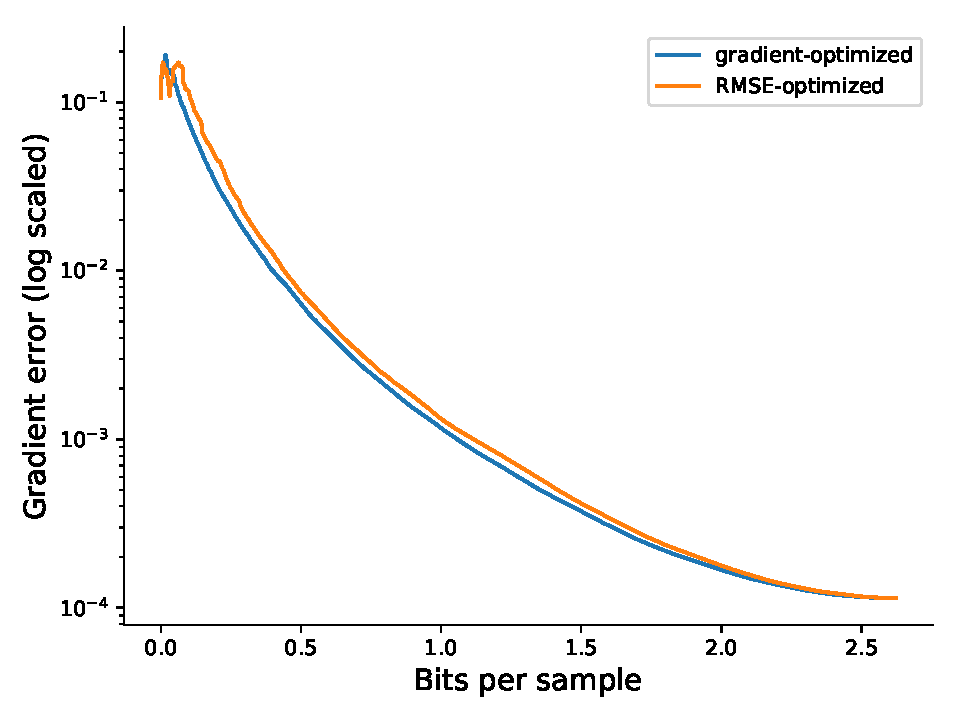
\includegraphics[width=0.48\linewidth]{img/gradient-laplacian/euler-gradient.pdf}}
	\subcaptionbox{magnetic}
	{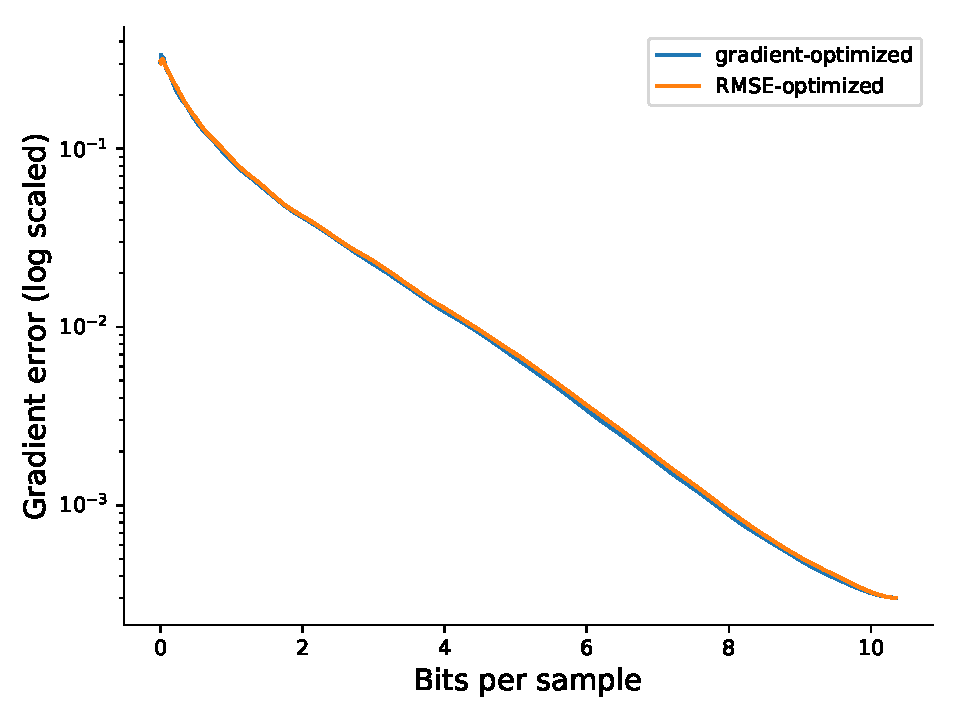
\includegraphics[width=0.48\linewidth]{img/gradient-laplacian/magnetic-gradient.pdf}}
	\subcaptionbox{diffusivity}
	{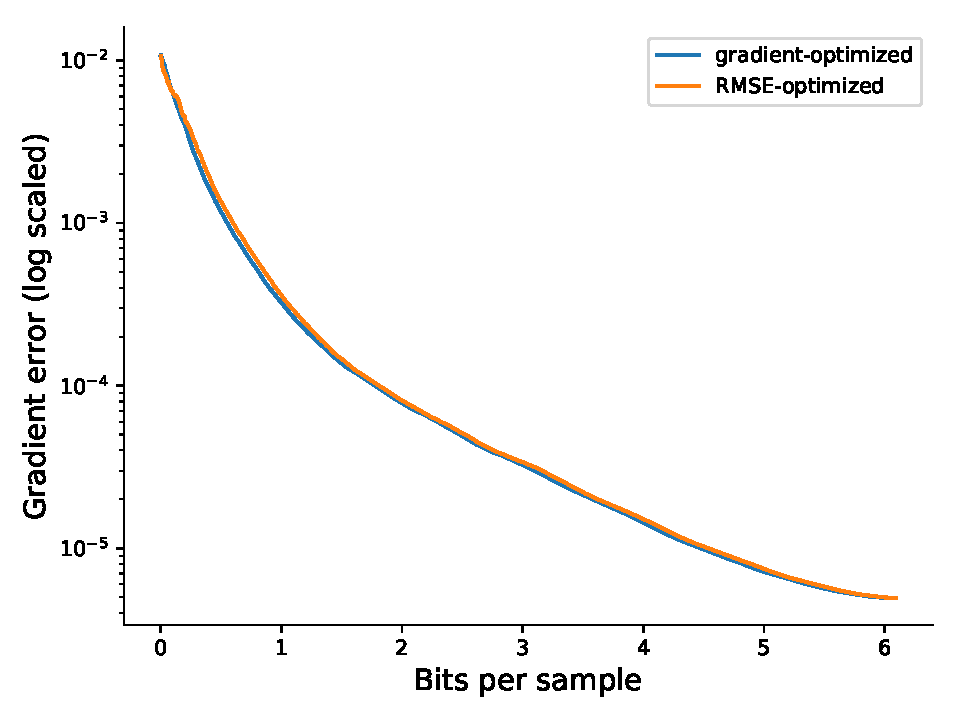
\includegraphics[width=0.48\linewidth]{img/gradient-laplacian/miranda-diffusivity-gradient.pdf}}
	\subcaptionbox{velocityx}
	{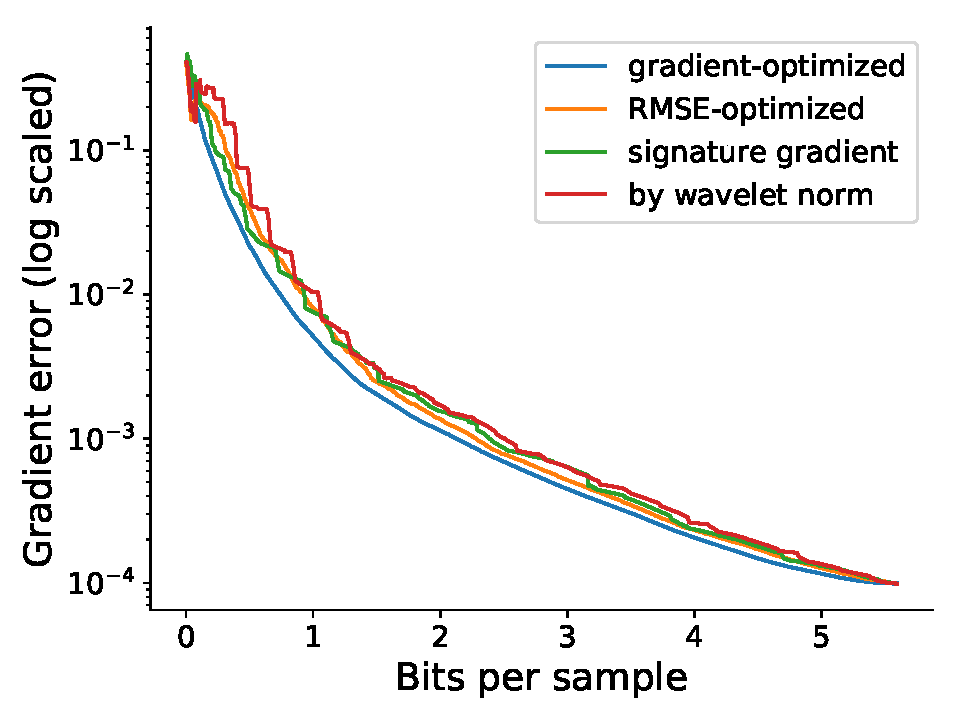
\includegraphics[width=0.48\linewidth]{img/gradient-laplacian/miranda-velocityz-gradient.pdf}}
	\caption{Gradient error comparison between \emph{gradient-optimized} and \emph{rmse-optimized}
	streams for four data sets. Smaller is better. Note that the leading zero chunks are still
	skipped.}
	\label{fig:gradient-error-comparison}
\end{figure}

Figure \ref{fig:gradient-error-comparison} suggests that the \emph{rmse-optimized} streams are also
nearly optimal for gradient computation. The gradient operator is not invertible, that is, there are
infinitely many functions that result in the same gradient field. So it is not surprising that the
two streams both produce the best possible gradient progression, but it is worth noting that only
the \emph{rmse-optimized} stream produces an accurate function as well. We give evidence to this
claim is in Figure \ref{fig:gradient-comparison}, in which we reconstruct the euler data at 0.25
bits per sample using both streams, and show the difference in gradient between the two. The two
gradient fields differ the most along very sharp edges, but are in general congruent (a), while
the \emph{rmse-optimized} stream produces significantly more accurate reconstruction of the function
itself (b, c, and d).

\begin{figure}
	\centering
	\subcaptionbox{gradient difference}
	{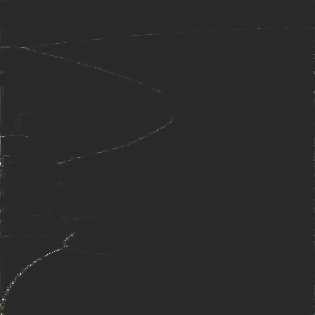
\includegraphics[width=0.24\linewidth]{img/gradient-laplacian/grad-diff.png}}
	\subcaptionbox{original data}
	{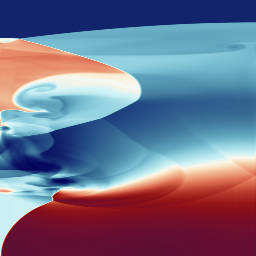
\includegraphics[width=0.24\linewidth]{img/gradient-laplacian/euler-original.png}}
	\subcaptionbox{\emph{rmse-optimized}}
	{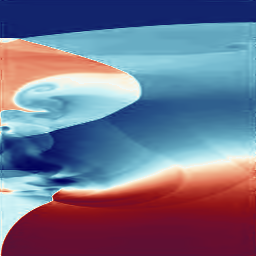
\includegraphics[width=0.24\linewidth]{img/gradient-laplacian/euler-rmse.png}}
	\subcaptionbox{\emph{gradient-optimized}}
	{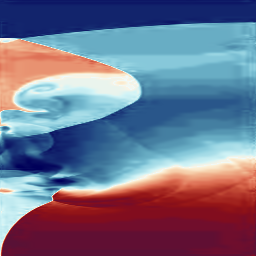
\includegraphics[width=0.24\linewidth]{img/gradient-laplacian/euler-gradient.png}}
	\caption{Comparing \emph{rmse-optimized} and \emph{gradient-optimized} at 0.25 bits per sample. }
	\label{fig:gradient-comparison}
\end{figure}

It is therefore reasonable in practice to simply use heuristics that are optimized for RMSE when the
analysis relies on an accurate gradient field. One such heuristic is the one used by the \emph{by
wavelet norm} stream (when coupled with a typical entropy compression that avoids most of the
leading zero bits).

\subsection{Laplacian}

For Laplacian, we use the three-point finite difference in each dimension separately:
$\frac{{\partial}^2}{\partial{x^2}}f(x,y) \approx f(x-1,y)-2f(x,y)+f(x+1,y)$, and $\Delta
f=(\frac{{\partial}^2}{\partial{x^2}}+\frac{{\partial}^2}{\partial{y^2}})f$. The Laplacian error is
defined as the RMSE between the reconstructed Laplacian scalar field and the original Laplacian
scalar field. Again, algorithm [REF] is used to compute a \emph{laplacian-optimized} bit stream that
minimizes this error. In Figure \ref{fig:laplacian-comparison} we compare this stream with the
\emph{rmse-optimized} stream using the PSNR of the difference in Laplacian (compared to the
ground truth) as the error metric. The stream labeled \emph{laplacian signature} is to be ignored for
now. (TODO: why is it in the plot? maybe do not mention it at all? or just say that it will be explained later)

\begin{figure}
	\centering
	\subcaptionbox{euler}
	{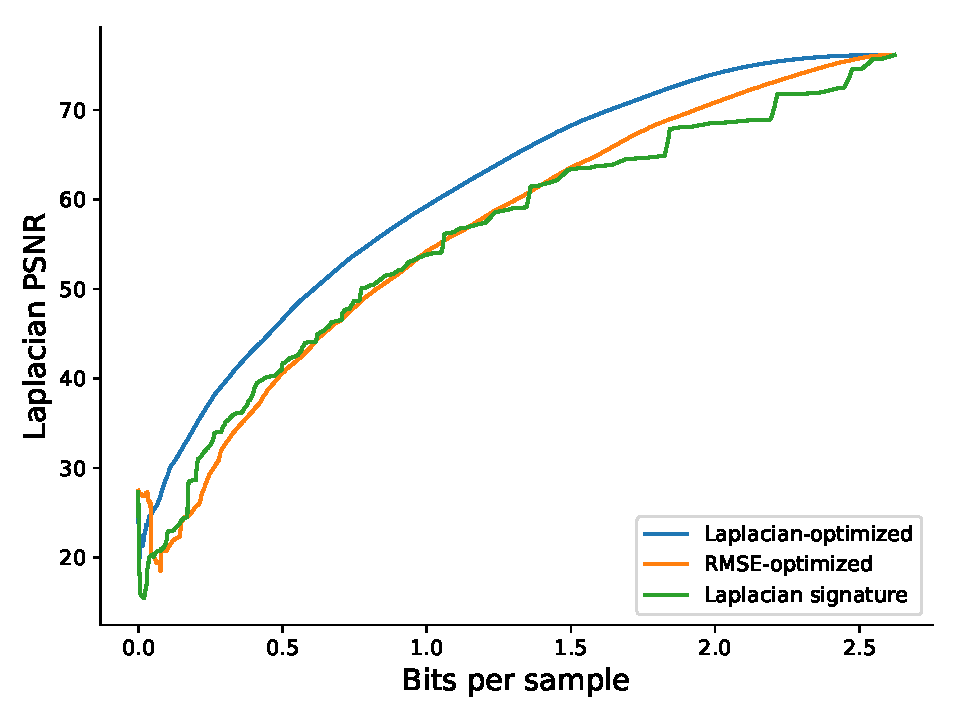
\includegraphics[width=0.48\linewidth]{img/gradient-laplacian/euler-laplacian.pdf}}
	\subcaptionbox{magnetic}
	{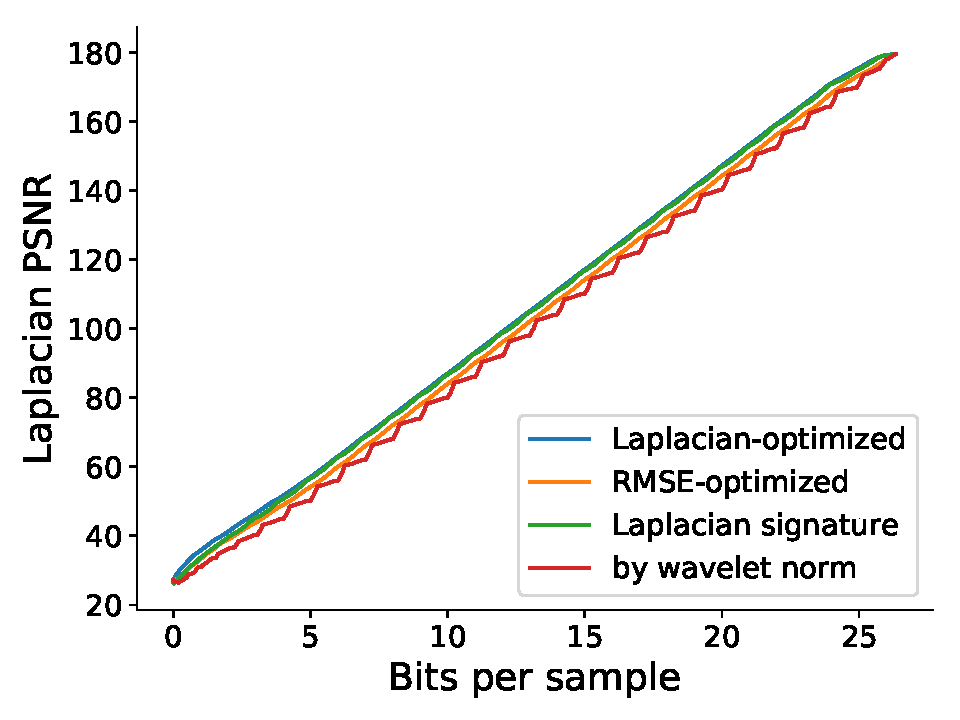
\includegraphics[width=0.48\linewidth]{img/gradient-laplacian/magnetic-laplacian.pdf}}
	\subcaptionbox{diffusivity}
	{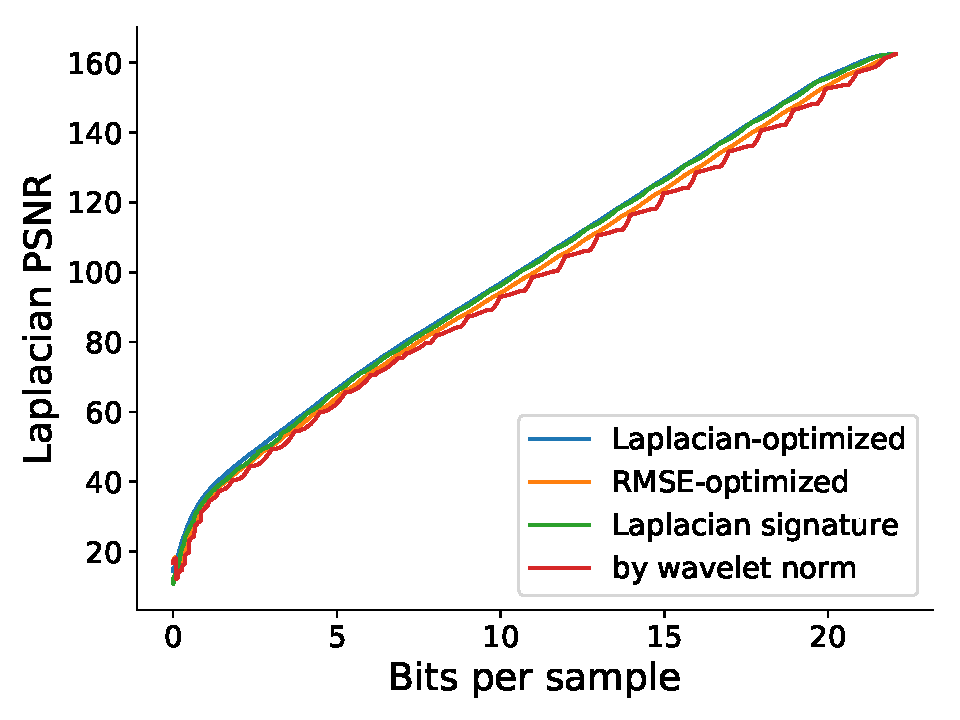
\includegraphics[width=0.48\linewidth]{img/gradient-laplacian/miranda-diffusivity-laplacian.pdf}}
	\subcaptionbox{velocityz}
	{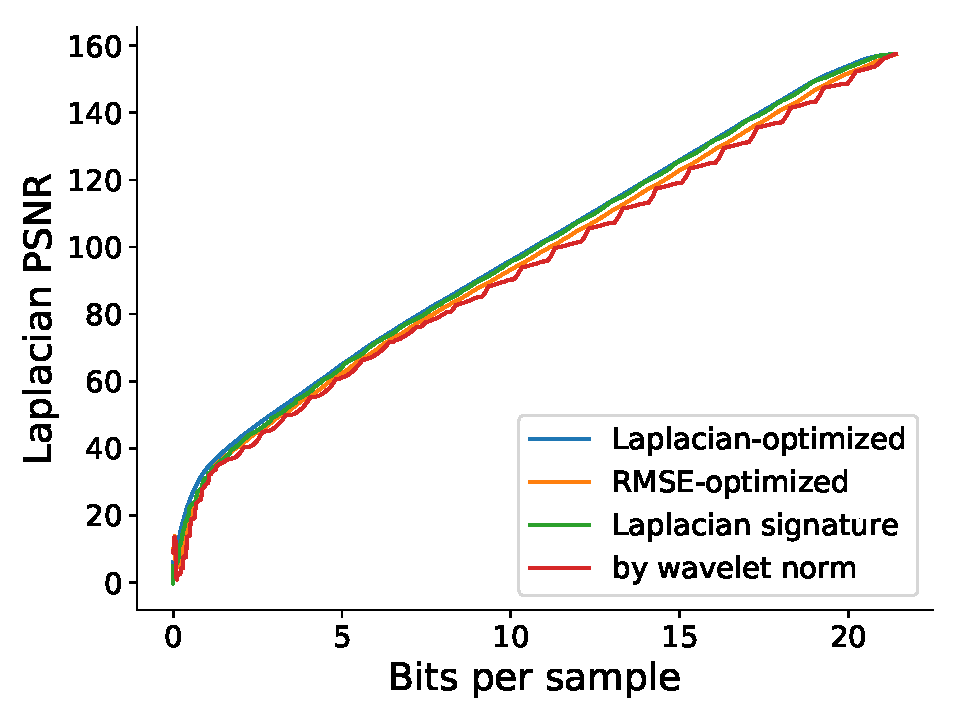
\includegraphics[width=0.48\linewidth]{img/gradient-laplacian/miranda-velocityz-laplacian.pdf}}
	\caption{Comparing \emph{rmse-optimized}, \emph{laplacian-optimized} and \emph{laplacian
	signature} streams in PSNR of Laplacian error (higher is better).}
	\label{fig:laplacian-comparison}
\end{figure}

It can be observed that unlike the case for gradient, there exists significant differences between
the \emph{rmse-optimized} and \emph{laplacian-optimized} streams with regards. To understand these
differences we plot the precision of every wavelet coefficients at a low bit rate in Figure
\ref{fig:laplacian-precision-comparison} (a and b). When cross refererencing this Figure with Figure
\ref{fig:gradient-comparison}b we see that the \emph{laplacian-optimized} stream priotizes
finer-resolution bits where the sharp shockwave is, unlike the \emph{rmse-optimized} stream which
prefers lower-ordered, coarse-resolution bits. This effect makes sense intuitively, as the
derivative operator makes functions less smooth, hence amplifing hard edges. This happens in the
gradient case too, but to a much lesser degree.

\begin{figure}
	\centering
	\subcaptionbox{\emph{laplacian-optimized}}
	{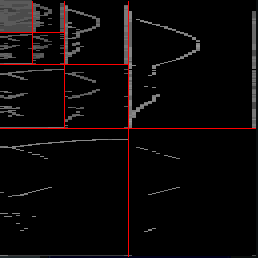
\includegraphics[width=0.32\linewidth]{img/gradient-laplacian/euler-prec-lap.png}}
	\subcaptionbox{\emph{rmse-optimized}}
	{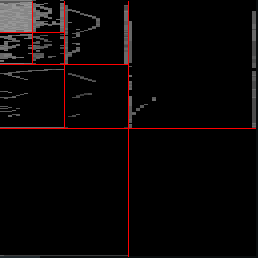
\includegraphics[width=0.32\linewidth]{img/gradient-laplacian/euler-prec-rmse.png}}
	\subcaptionbox{\emph{laplacian signature}}
	{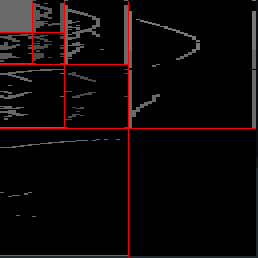
\includegraphics[width=0.32\linewidth]{img/gradient-laplacian/euler-prec-signature.png}}
	\caption{Precision distribution of wavelet coefficients at 0.25 bits per sample for the euler data
	set. Each square box with red boundary is a wavelet subband (the coarsest subband is in the top
	left). Brighter pixels correspond to higher-precision wavelet coefficients (black means no bit of
	that coefficient has not been received, while white means the whole coefficient has been
	received).}
	\label{fig:laplacian-precision-comparison}
\end{figure}

To capture the core characteristics of the \emph{laplacian-optimized} stream, we introduce the
concept of a stream \emph{signature}. A signature is a matrix with $B$ columns and $L$ rows, with
$B$ being the number of bit planes in the data set, and $L$ being the number of subbands in the
wavelet transform. Each cell $(b,l)$ in the signature matrix contains a value in the range
$[0,B\times L)$, and the ordering of these values reflects the relative ordering in which the $b$
bit on subband $l$ (for all $l$ and $b$) appear in the stream, on average. The signatures for
\emph{rmse-optimized}, \emph{laplacian-optimized}, and also \emph{gradient-optimized} for the euler
data set are visualized in Figure \ref{fig:signature-comparison}. 

\begin{figure}
	\centering
	\subcaptionbox{\emph{rmse-optimized}}
	{
\includegraphics[width=0.32\linewidth]{img/gradient-laplacian/SIG-GREEDY-(rmse).png}}
	\subcaptionbox{\emph{laplacian-optimized}}
	{
\includegraphics[width=0.32\linewidth]{img/gradient-laplacian/SIG-GREEDY-(laplacian).png}}
	\subcaptionbox{\emph{gradient-optimized}}
	{
\includegraphics[width=0.32\linewidth]{img/gradient-laplacian/SIG-GREEDY-(gradient).png}}
	\caption{Stream signatures visualized through a linear-blue color map (brighter is higher
	priority). From left to right: higher-ordered to lower-ordered bit planes. From top to bottom:
	coarser to finer subbands. Note that the streams from which the signatures are extracted do not
	contain leading zero bits, which explains the very dark cells }
	\label{fig:signature-comparison}
\end{figure}

The algorithm used to compute a signature from a stream is presented below (TODO: placeholder).
\begin{algorithm}
  \KwData{this text}
  \KwResult{how to write algorithm with \LaTeX2e }
  initialization\;
  \While{not at end of this document}{
   read current\;
   \eIf{understand}{
    go to next section\;
    current section becomes this one\;
    }{
    go back to the beginning of current section\;
   }
  }
  \caption{How to write algorithms}
 \end{algorithm}

Using the signature for \emph{laplacian-optimized}, we are able construct a data-independent stream
(in the sense that once the signature is computed and is given, the ordering of the bits follows the
the signature only). This stream, called \emph{laplacian signature}, performs at least as well as,
and often better, than \emph{rmse-optimized} for all data sets (see Figure
\ref{fig:laplacian-comparison}). The reason \emph{laplacian signature} does not always outperform
\emph{rmse-optimized}, and that there is still a gap between itself and \emph{laplacian-optimized}
is that the signature is computed essentially by `'averaging'' local signatures, a process that
lessen the effectiveness of the signature when the data is highly inhomogenous (e.g., the euler data
set with its sharp shockwaves). Nevertheless, even with one signature for the whole domain, we are
able to reconstruct more accurate Laplacian in all cases in experiment. In practice, the signature
is a tiny piece of meta information that can be pre-computed, stored, and transmitted before any
value bits to help `'steer'' the data stream, whenever Laplacian is the quantity of interest.
